\scanpage{83}
% archive sheet number: 82
% Long oblique strokes cancel this draft.
\deleted{IV 7.5.}

\deleted{I am still not very happy with the latest version, for one does not state what one really proves, and consequently there are cases (such as the ``$\text{\unsure{\rlap{p}c}\unsure{\rlap{r}o}p\rlap{f}rof}\quad n$'', or ``in\rlap{e}tegral'') which escape the statement as it is given, but are included in the proof. So I propose to restate things as follows:}

\deleted{\uline{Theorem} 7.5.1.\quad Let $A\quad B$ be a local homomorphism of noetherian local rings, $\text{\uuline{R}}(C)$ a property \deleted{of local rings} involving an argument which i s a noe\rlap{h}t\unsure{\rlap{t}h|h}erian local ring. We suppose\deleted{\unsure{x|r}} that $(B,R)$ satisfies :}

\deleted{a) For every ring \mbox{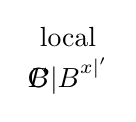
\begin{tikzpicture}[baseline=(base.base)]
\node[inner sep=0] (base) {$\text{\unsure{\rlap{C}B|B}}^{\deleted{\unsure{x|'}}}$};
\node[anchor=south,inner sep=0,yshift=.12cm] at (base.north) {\inserted{local}};
\end{tikzpicture}} which is a localization of a finite $B$-algebra, and every regular element $t\quad\underline{r}(C)$, $\text{\uuline{R}}(C/tC)$ implies $\text{\uuline{R}}(C)$.}

\deleted{b) If $C$ is a finite $B$-algebra, then $U_{\text{\uuline{R}}}(\operatorname{Spec}(C))$ is open.}

\deleted{We suppose moreover that $A$ satisfies the following conditions\deleted{\unsure{x}} (satisfied if $A$ is ``excellent'' (7.8.2.) in particular if $A$ is complete):}

\deleted{\handwritten{$\alpha$}) $A$ is \mbox{
\begin{tikzpicture}[baseline=(word.base)]
\node[inner sep=0] (word) {universally};
% Thin shallow curved trace below the first half; no textual value or origin assigned.
\draw[line width=.3pt,opacity=.6] ([xshift=.30cm,yshift=-.13cm]word.south west) .. controls ([xshift=.65cm,yshift=-.32cm]word.south west) and ([xshift=1.25cm,yshift=-.35cm]word.south west) .. ([xshift=1.65cm,yshift=-.31cm]word.south west);
\end{tikzpicture}} Japanese.}

\deleted{\handwritten{$\beta$}) For every finite integral algebra $C$ over $A$, $\operatorname{Spec}(C)$ contains a nonempty open subset which is regular,}

\deleted{\mbox{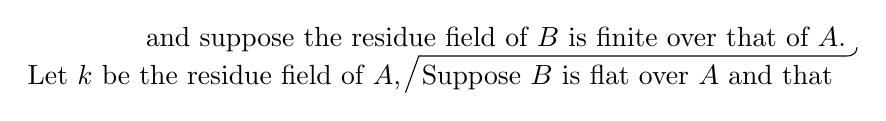
\begin{tikzpicture}[baseline=(left.base)]
\node[inner sep=0] (left) {Let $k$ be the residue field of $A$,};
\node[anchor=base west,inner sep=0,xshift=.25cm] (right) at (left.base east) {Suppose $B$ is flat over $A$ and that};
\node[anchor=south west,inner sep=0,xshift=1.5cm,yshift=.15cm] (added) at (left.north west) {\inserted{and suppose the residue field of $B$ is finite over that of $A$.}};
\path (added.south west) -- coordinate[pos=.39] (bend) (added.south east);
\draw ([xshift=.05cm,yshift=-.03cm]left.south east) -- ([yshift=-.04cm]bend) -- ([yshift=-.04cm]added.south east) .. controls ([xshift=.09cm,yshift=-.04cm]added.south east) and ([xshift=.13cm,yshift=.01cm]added.south east) .. ([xshift=.13cm,yshift=.07cm]added.south east);
\end{tikzpicture}} $B\otimes_A k$ over $k$ satisfies the condition ``geometric $Q$''; \rlap{t}Then all the fibers of $\operatorname{Spec}(B)$ over $\operatorname{Spec}(A)$ satisfy the geometric $Q$ condition.}

\deleted{Proof. The hypotheses made on $A\quad B$ are stable under finite base change $A\quad A'$, provided one takes care to ref\unsure{\rlap{r}o}rmulate the hypotheses for semi-local $A,B$, the homomorphism $A\quad B$ semi-local (i.e. the inverse image of a maximal ideal is a maximal ideal) and replaces the residue field of $A$ by the residue fields of $A$. \deleted{(NB then} (NB this extension does not deserve to appear in the statement of the theorem, it is just a technical intermediate step for the proof). One is thus reduced to the case $A$ integral and to seeing that the generic fiber satisfies}
